% Drawing 156-9/01-3 -- folder 156-9, batch 01, archive page 3 (PDF page 4).
% Transcription: un graphe orienté, les flèches montant vers le haut (traits doublés à l'encre brune), avec hachures au crayon dans deux bandes. Au sommet G $(\mathcal{A})$. Au-dessous, à gauche S $(\Sigma$ ou $\mathcal{A})$ cerclé, au milieu F, à droite L ; sur l'arête de L à G un point « Div » ; sur l'arête de SF à S une marque « [S Div] ». Au niveau suivant SF, LS $(\Sigma$ ou $\mathcal{L})$ (cerclé) et FL $=$ P. Puis FLS $=$ E $(\mathcal{L})$ au centre et M (cerclé) à gauche. Puis Mq (sous M) et EM (cerclé, sous E). En bas D, recevant deux flèches venues de v et de p. Flèches : S, F, L $\to$ G ; SF $\to$ S et F ; LS $\to$ S et L ; P $\to$ F et L ; E $\to$ SF, LS, P ; M $\to$ SF ; Mq $\to$ M ; EM $\to$ M et E ; D $\to$ Mq et EM ; v, p $\to$ D. Pointillés de S à Div et de F à L.
% Kind: oriented graph (lattice of atelier types). Method 2 (schematic redraw from the facsimile). Status: ok.
% Notes: Oriented graph, arrows upwards (ink lines doubled in brown, drawn once): G (A) at the top; S (Sigma or A) ringed, F, L; Div on the edge L - G; [S Div] on the edge SF - S side; SF, LS (Sigma or L) ringed, FL = P; FLS = E (L) and M ringed; Mq and EM ringed; D, receiving the arrows from v and p. Arrows S, F, L -> G; SF -> S, F; LS -> S, L; P -> F, L; E -> SF, LS, P; M -> SF; Mq -> M; EM -> M, E; D -> Mq, EM; v, p -> D. The dotted strokes (S to Div, F to L side) are dashed here; the two hatched bands are pencil hatching. The notes in the left margin and below the graph are text and left out.
% Coordinates: 1 unit = 1 mm = 1/100 of the crop width (bbox in page fractions: [0.52, 0.12, 0.84, 0.5]).
% Redrawn by Claude (claude-opus-5-5), issue #73, 2026-11-07; not checked by a human; not compiled (no TeX in the session).
% Rights: reproduces part of the work -- behind RENDER_TRANSCRIPTS, never published by itself.
\documentclass[tikz,border=3pt]{standalone}
\usepackage{amsmath,amssymb}
\usetikzlibrary{patterns,arrows.meta}
\tikzset{pencil/.style={black!45}, struck/.style={black!35}, mark/.style={circle,draw,inner sep=1.3pt}, pt/.style={circle,fill,inner sep=0.9pt}, opt/.style={circle,draw,fill=white,inner sep=1.1pt}}
\begin{document}
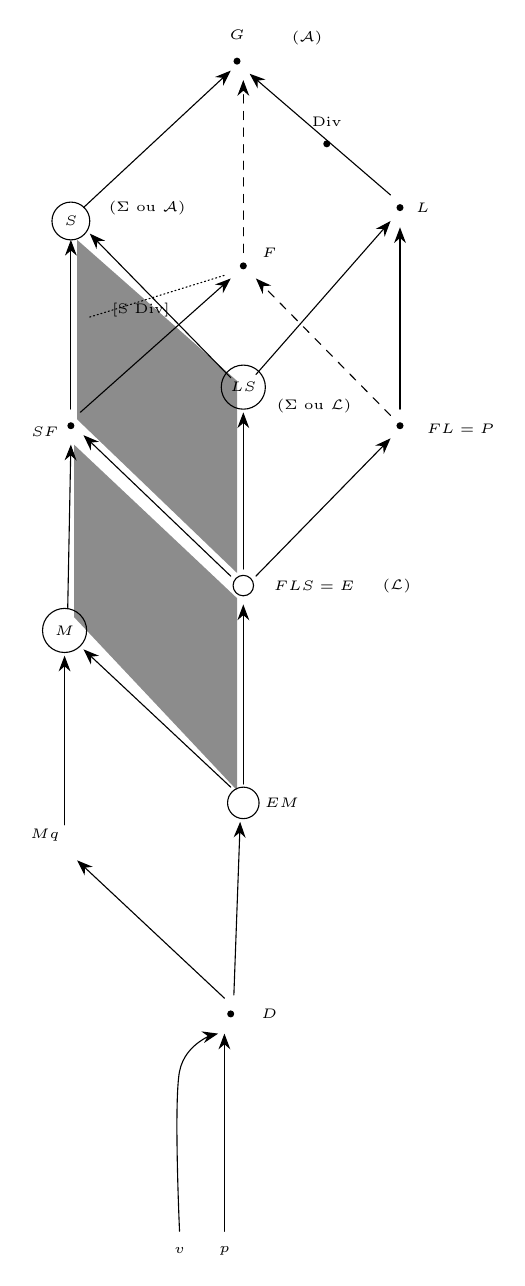
\begin{tikzpicture}[x=1mm,y=1mm,line cap=round,line join=round,font=\scriptsize]
\fill[pattern=north east lines,pencil] (38.2,-32.5) -- (58.5,-50.4) -- (58.5,-74.8) -- (38.2,-55.3) -- cycle;
\fill[pattern=north east lines,pencil] (37.8,-58.5) -- (58.5,-78) -- (58.5,-102.4) -- (37.8,-80.4) -- cycle;
\draw[-{Stealth[length=2mm]}] (39,-28.4) -- (57.7,-11);
\draw[-{Stealth[length=2mm]},dashed] (59.3,-34.1) -- (59.3,-12.2);
\draw[-{Stealth[length=2mm]}] (78,-26.8) -- (60.1,-11.4);
\node[pt] at (69.9,-20.3) {};
\node[inner sep=1pt] at (69.9,-17.5) {\tiny Div};
\draw[-{Stealth[length=2mm]}] (37.4,-54) -- (37.4,-32.5);
\draw[-{Stealth[length=2mm]}] (38.6,-54.4) -- (57.7,-37.4);
\draw[-{Stealth[length=2mm]}] (57.7,-50) -- (39.8,-31.7);
\draw[-{Stealth[length=2mm]}] (60.9,-49.6) -- (78,-30.1);
\draw[-{Stealth[length=2mm]},dashed] (78,-54.8) -- (60.9,-37.4);
\draw[-{Stealth[length=2mm]}] (79.2,-54) -- (79.2,-30.9);
\draw[densely dotted] (39.8,-42.3) -- (56.9,-37);
\node[inner sep=1pt] at (46.3,-41.4) {\tiny [S Div]};
\draw[-{Stealth[length=2mm]}] (57.7,-75.2) -- (39,-57.3);
\draw[-{Stealth[length=2mm]}] (59.3,-74.3) -- (59.3,-54.4);
\draw[-{Stealth[length=2mm]}] (60.9,-75.2) -- (78,-57.7);
\draw[-{Stealth[length=2mm]}] (37,-79.2) -- (37.4,-58.5);
\draw[-{Stealth[length=2mm]}] (36.6,-106.8) -- (36.6,-85.3);
\draw[-{Stealth[length=2mm]}] (57.7,-102) -- (39,-84.5);
\draw[-{Stealth[length=2mm]}] (59.3,-101.6) -- (59.3,-78.8);
\draw[-{Stealth[length=2mm]}] (56.9,-128.8) -- (38.2,-111.3);
\draw[-{Stealth[length=2mm]}] (58.1,-128.4) -- (58.9,-106.4);
\draw[-{Stealth[length=2mm]}] plot[smooth, tension=0.55] coordinates {(51.2,-158.4) (51.2,-138.1) (56.1,-133.3)};
\draw[-{Stealth[length=2mm]}] (56.9,-158.4) -- (56.9,-133.3);
\node[pt] at (58.5,-9.8) {};
\node[pt] at (59.3,-35.8) {};
\node[pt] at (79.2,-28.4) {};
\node[pt] at (79.2,-56.1) {};
\node[pt] at (37.4,-56.1) {};
\node[pt] at (57.7,-130.8) {};
\draw (37.4,-30.1) circle[radius=2.4];
\draw (59.3,-51.2) circle[radius=2.8];
\draw (59.3,-76.4) circle[radius=1.3];
\draw (36.6,-82.1) circle[radius=2.8];
\draw (59.3,-104) circle[radius=2];
\node[inner sep=1pt] at (58.5,-6.5) {\tiny $G$};
\node[inner sep=1pt] at (67.4,-6.9) {\tiny $(\mathcal A)$};
\node[inner sep=1pt] at (37.4,-30.1) {\tiny $S$};
\node[inner sep=1pt] at (47.1,-28.4) {\tiny $(\Sigma$ ou $\mathcal A)$};
\node[inner sep=1pt] at (62.6,-34.1) {\tiny $F$};
\node[inner sep=1pt] at (82.1,-28.4) {\tiny $L$};
\node[inner sep=1pt] at (34.1,-56.9) {\tiny $SF$};
\node[inner sep=1pt] at (59.3,-51.2) {\tiny $LS$};
\node[inner sep=1pt] at (68.3,-53.6) {\tiny $(\Sigma$ ou $\mathcal L)$};
\node[inner sep=1pt] at (86.9,-56.5) {\tiny $FL=P$};
\node[inner sep=1pt] at (68.3,-76.4) {\tiny $FLS=E$};
\node[inner sep=1pt] at (78.8,-76.4) {\tiny $(\mathcal L)$};
\node[inner sep=1pt] at (36.6,-82.1) {\tiny $M$};
\node[inner sep=1pt] at (34.1,-108.1) {\tiny $Mq$};
\node[inner sep=1pt] at (64.2,-104) {\tiny $EM$};
\node[inner sep=1pt] at (62.6,-130.8) {\tiny $D$};
\node[inner sep=1pt] at (51.2,-160.9) {\tiny $v$};
\node[inner sep=1pt] at (56.9,-160.9) {\tiny $p$};
\end{tikzpicture}
\end{document}
